\problemname{KATT och råtta}
\noindent
En speciell typ av muterade jätteråttor har tagit över Göteborgs kloaker,
och stadsledningen har bett dig om hjälp med att lösa problemet.

Kloaken består av $N$ brunnar numrerade från $1$ till $N$, med $N-1$ rör som kopplar samman brunnarna.
Varje rör går mellan två brunnar, och kloaken är utformad
så att det går att färdas mellan varje par av brunnar genom att gå igenom en sekvens av rör.
För att dra ner på kostnaderna har man avskedat alla kloak-utvecklare i Göteborg, 
och man råkade därigenom lämna kloaksystemet helt odokumenterat.
Nu finns det alltså ingen kvar som vet mellan vilka par av brunnar det finns rör.

Det finns $K$ stycken jätteråttor, som befinner sig i olika brunnar.
Eftersom råttorna är så stora och aggresiva kan det aldrig vara två råttor i samma brunn.
Du har redan placerat ut $K$ stycken KATT:er (Kraftfull Atombaserad Träffsäker Torped) i olika brunnar.
Dessa kan du aktivera med ett enkelt knapptryck,
och du vill nu försöka få råttorna att gå till de brunnar där det finns KATT:er.
Men råttorna är väldigt intelligenta, och om inte alla KATT:er aktiveras samtidigt så kommer råttorna
lära sig att använda KATT:erna emot dig.

För att få råttorna att röra sig har du en stor mängd UGGL:or 
(Utropande Generator av Galna Ljud),
som spelar låtar som är särskilt irriterande för muterade jätteråttor.
Du får, i flera omgångar, välja en delmängd av brunnarna, och placera en UGGL:a i varje brunn i delmängden.
Alla råttor kommer sedan eventuellt springa ett rör för att undvika ljudet.
Mer specifikt kommer varje råtta att få möjligheten att fly från UGGL:orna,
och på grund av fysikens lagar kommer råttorna att göra detta i ordning av numret på brunnen de befinner sig i just nu.
Alltså, om det finns råttor i brunn $1$ och $2$ så kommer råttan i brunn $1$ att försöka fly först.
När denna råtta flytt färdigt kommer råttan i brunn $2$ att utföra sin flykt.
Råttorna vill maximera avståndet till närmsta UGGL:a.
En råtta kommer överväga att röra sig till alla brunnar, fria från andra råttor, 
inom ett rörs avstånd från där de befinner sig just nu.
Om ingen av dessa brunnar har ett strikt större avstånd till närmsta UGGL:a kommer råttan att stanna där den befinner sig nu. 
Annars kommer den att gå till den närliggande brunn med högst avstånd till närmsta UGGL:a.
Om det finns flera sådana brunnar väljer råttan brunnen med lägst nummer.
Avståndet mellan två brunnar är det minsta antalet rör du måste gå igenom för att färdas mellan dem.

Du har fått väldigt många UGGL:or av Göteborgs stad, men du hinner bara göra $25000$ omgångar av utplaceringar av UGGL:or innan 
råttornas parningssäsong (som skulle få ödesdigra konsekvenser!) börjar. I varje omgång får du placera UGGL:or i flera brunnar.


\section*{Interaktion}
Först ska ditt program läsa in talen $N$ ($2 \leq N \leq 100$) och $K$ ($1 \leq K < N$) som ut på en rad.
Sedan följer en rad med $K$ olika tal $1 \leq r_1 < ... < r_K \leq N$, som beskriver numren på de brunnar där det från början finns råttor.
Därefter skrivs ytterligare en rad med $K$ olika tal $1 \leq t_1 < ... < t_K \leq N$, som beskriver numren på de brunnar där du har placerat KATT:er.

När du vill göra en placering av UGGL:or ska du först skriva ut ett tal $M$, antalet UGGL:or du placerar ut. 
Därefter ska du, på samma rad, skriva talen $1 \leq s_1 < ... < s_M \leq N$,
de brunnar där du vill placera UGGL:or. En UGGL:a får placeras i en brunn oavsett om det finns en råtta där eller inte.
Sedan ska ditt program läsa en rad med $K$ tal, $1 \leq r_1 < ... < r_K \leq N$, 
de brunnar där det finns råttor efter att alla råttor försökt fly från UGGL:orna.

När du lyckats få alla råttor till brunnar med fällor i ska du skriva ut ``\texttt{activate!}'' på en rad. 
Ditt program ska då avslutas.

\textbf{Se till att flusha outputen efter varje query}, annars kan du få \textit{Time Limit Exceeded}.
I C++ kan detta göras med exempelvis \texttt{cout << flush;}
eller \texttt{fflush(stdout);},
i Python med \texttt{stdout.flush()}
och i Java med \texttt{System.out.flush();}.
Kloaken är är inte nödvändigtvis slumpmässigt genererad. 
Det är dock garanterat att råttor startar på, och KATT:er är utplacerade på, uniformt slumpmässigt utvalda brunnar. 
Domaren är inte adaptiv, vilket betyder att det är bestämt på förhand hur kloaken ser ut.

För att förenkla testning av ditt program tillhandahåller vi ett verktyg som du kan ladda ner längst ned
vid ``attachments'' på det här problemets Kattissida. Se kommentaren högst upp i filen för en beskrivning av hur det kan användas.

\section*{Poängsättning}
Din lösning kommer att testas på en mängd testfallsgrupper.
För att få poäng för en grupp så måste du klara alla testfall i gruppen.

\noindent
\begin{tabular}{| l | l | l |}
  \hline
  \textbf{Grupp} & \textbf{Poäng} & \textbf{Gränser} \\ \hline
  $1$   & $5$        & $N = 2$ \\ \hline
  $2$   & $5$        & $N \leq 3$ \\ \hline
  $3$   & $9$        & $N \leq 10$ \\ \hline
  $4$   & $20$        & $K = 1$ \\ \hline
  $5$   & $15$        & Det går ett rör mellan brunn $i$ och brunn $i+1$ för alla $1 \leq i < N$. \\ \hline
  $6$   & $21$        & $N \leq 50$ \\ \hline
  $7$   & $25$        & Inga ytterliga begränsningar. \\ \hline
\end{tabular}


\section*{Förklaring av exempelfall 2}

\begin{centering}
  \begin{figure}[h]
    \centering
    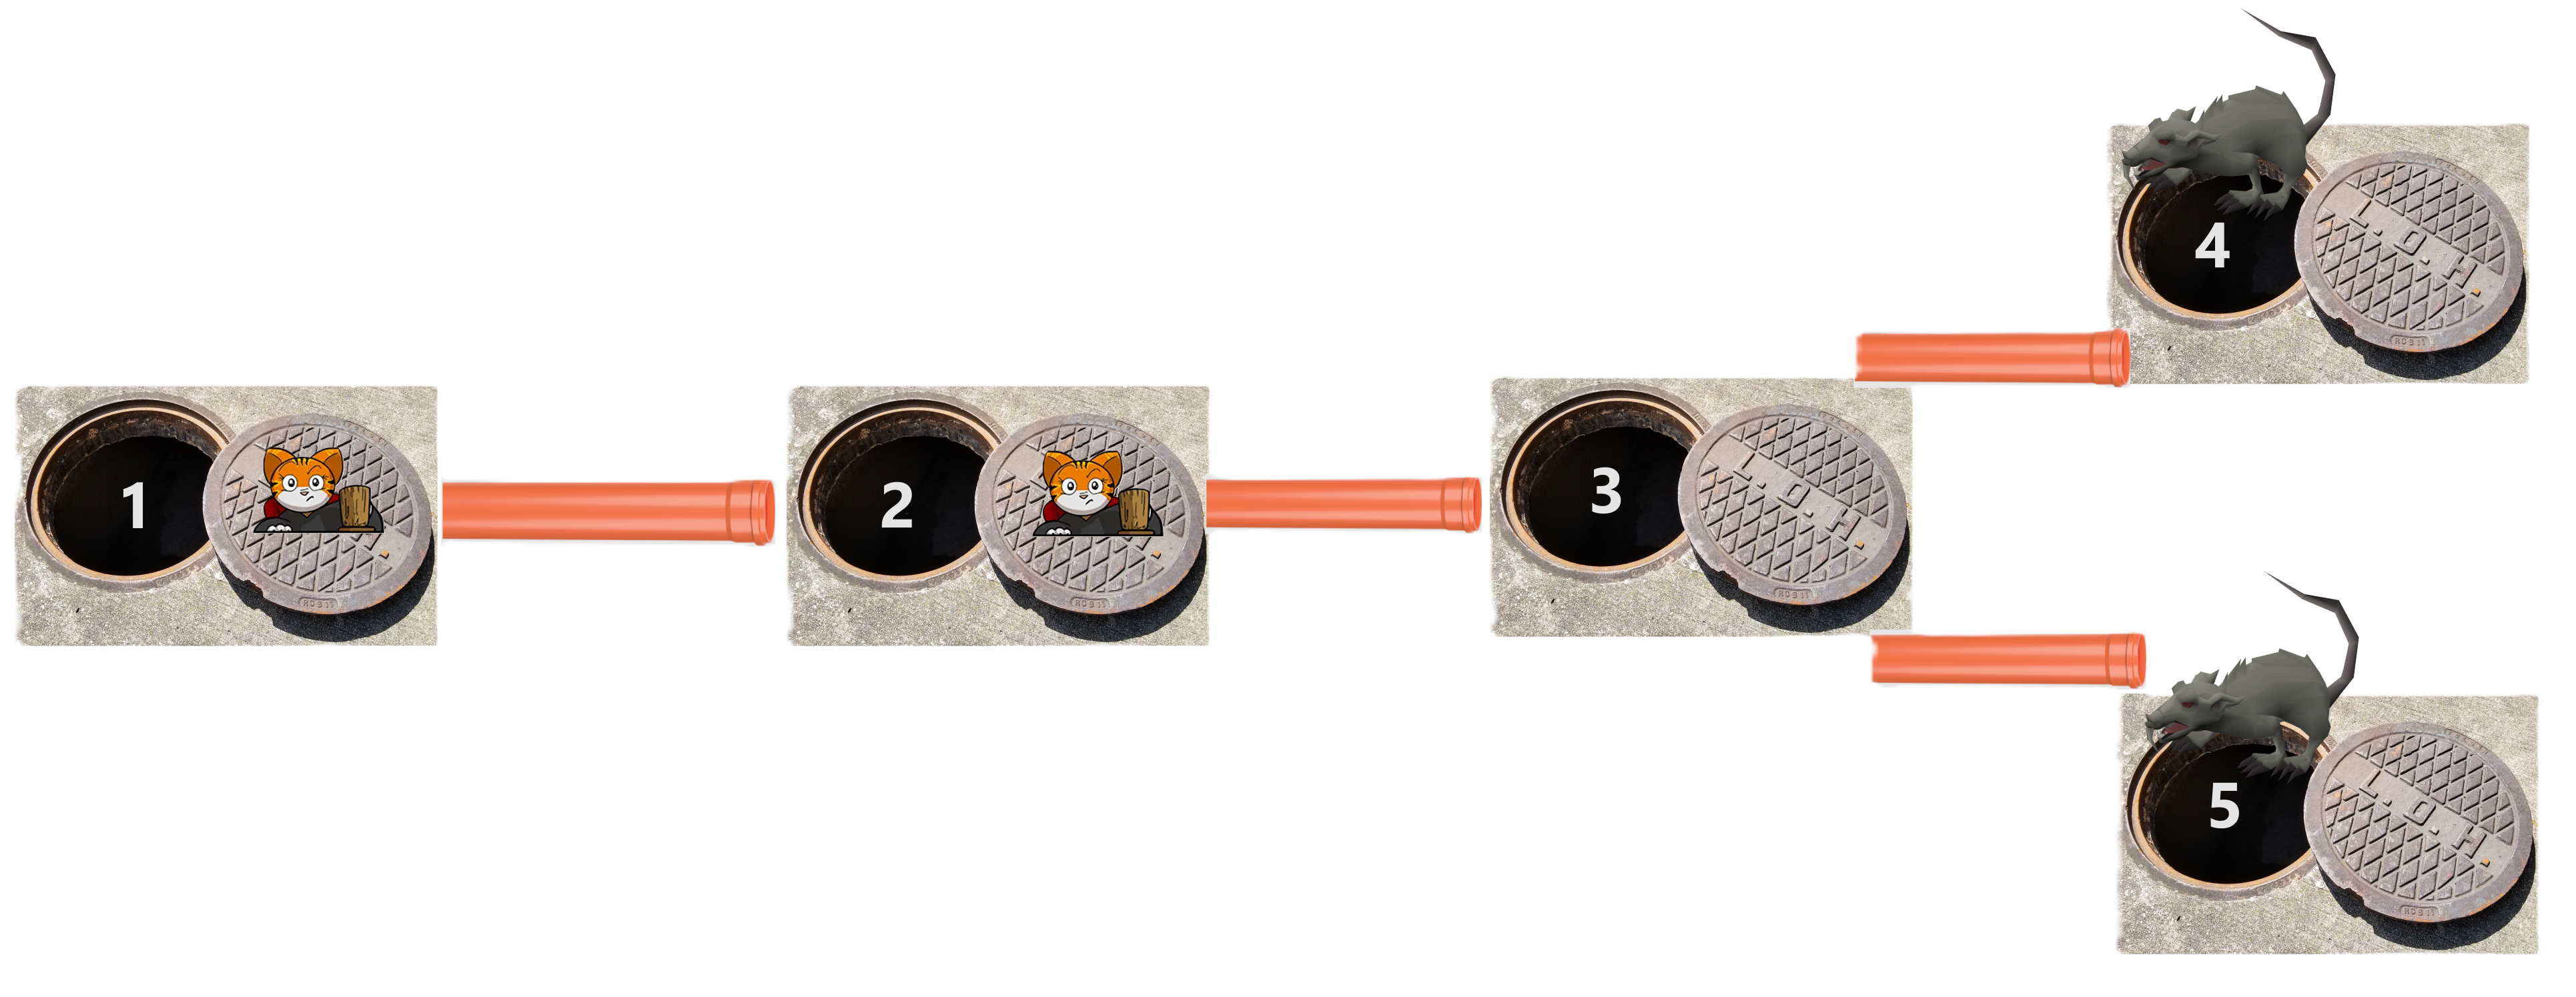
\includegraphics[scale=0.2]{rats_graph before.png}
    \caption{Kloakens utseende i exempelfall 2. Observera att ditt program inte vet vart rören går.}
  \end{figure}
\end{centering}

\begin{centering}
  \begin{figure}[h]
    \centering
    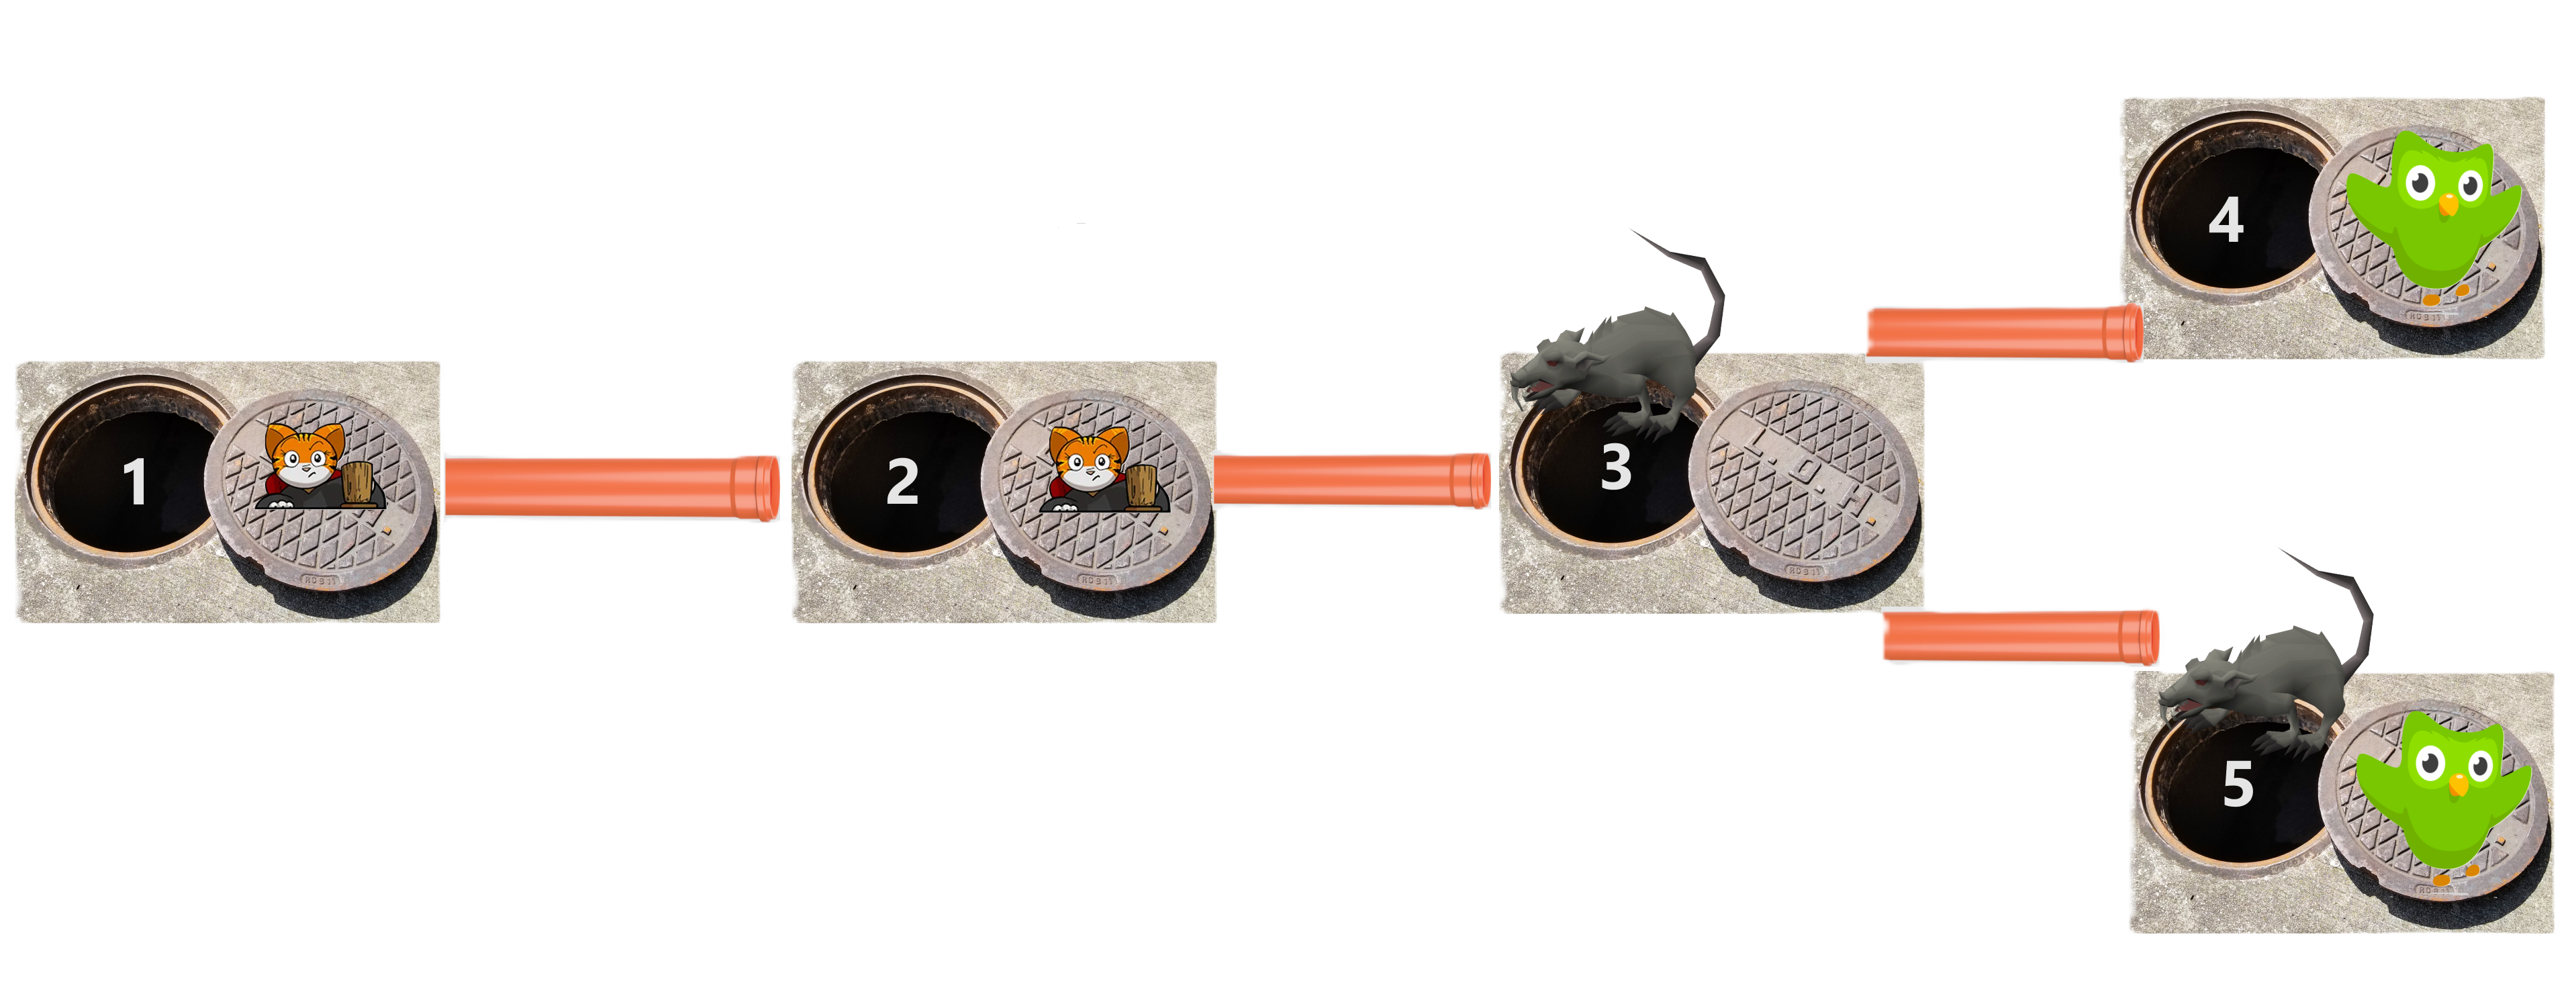
\includegraphics[scale=0.2]{rats_graph step1.png}
    \caption{När du placerar UGGL:or i brunnar $4$ och $5$ kommer båda dessa råttor att bli mycket störda. Råttan i brunn $4$ får chans att fly först, eftersom $4 < 5$, och den flyr till brunn $3$. När råttan i brunn $5$ sedan försöker fly finns det ingen ledig brunn att välja.}
  \end{figure}
\end{centering}

\begin{centering}
  \begin{figure}[h]
    \centering
    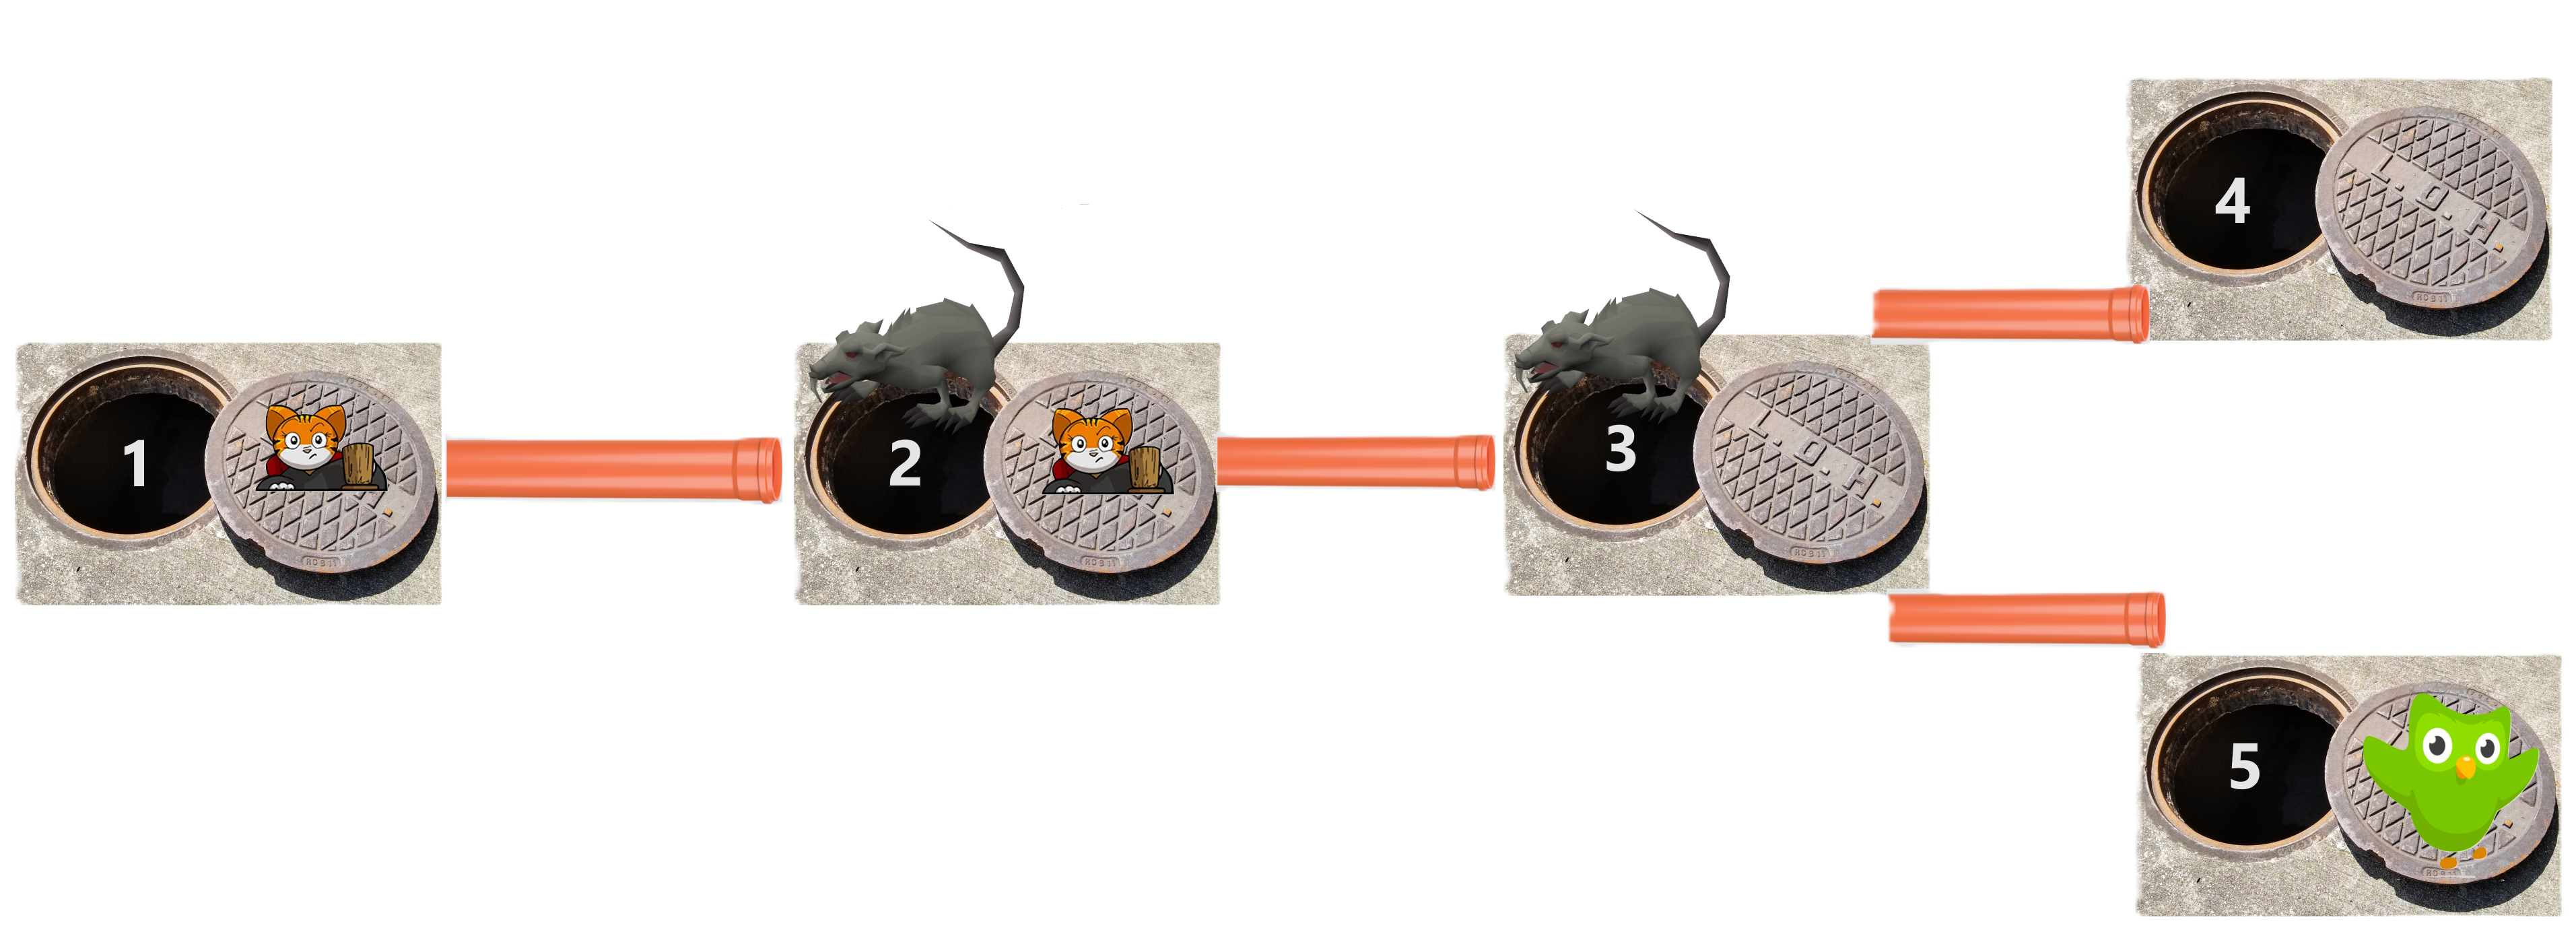
\includegraphics[scale=0.2]{rats_graph step2.png}
    \caption{När du placerar en ensam UGGL:a i brunn $5$ flyr först råttan i brunn $3$ till brunn $2$, och råttan i brunn $5$ flyr sedan till brunn $3$.}
  \end{figure}
\end{centering}

\begin{centering}
  \begin{figure}[h]
    \centering
    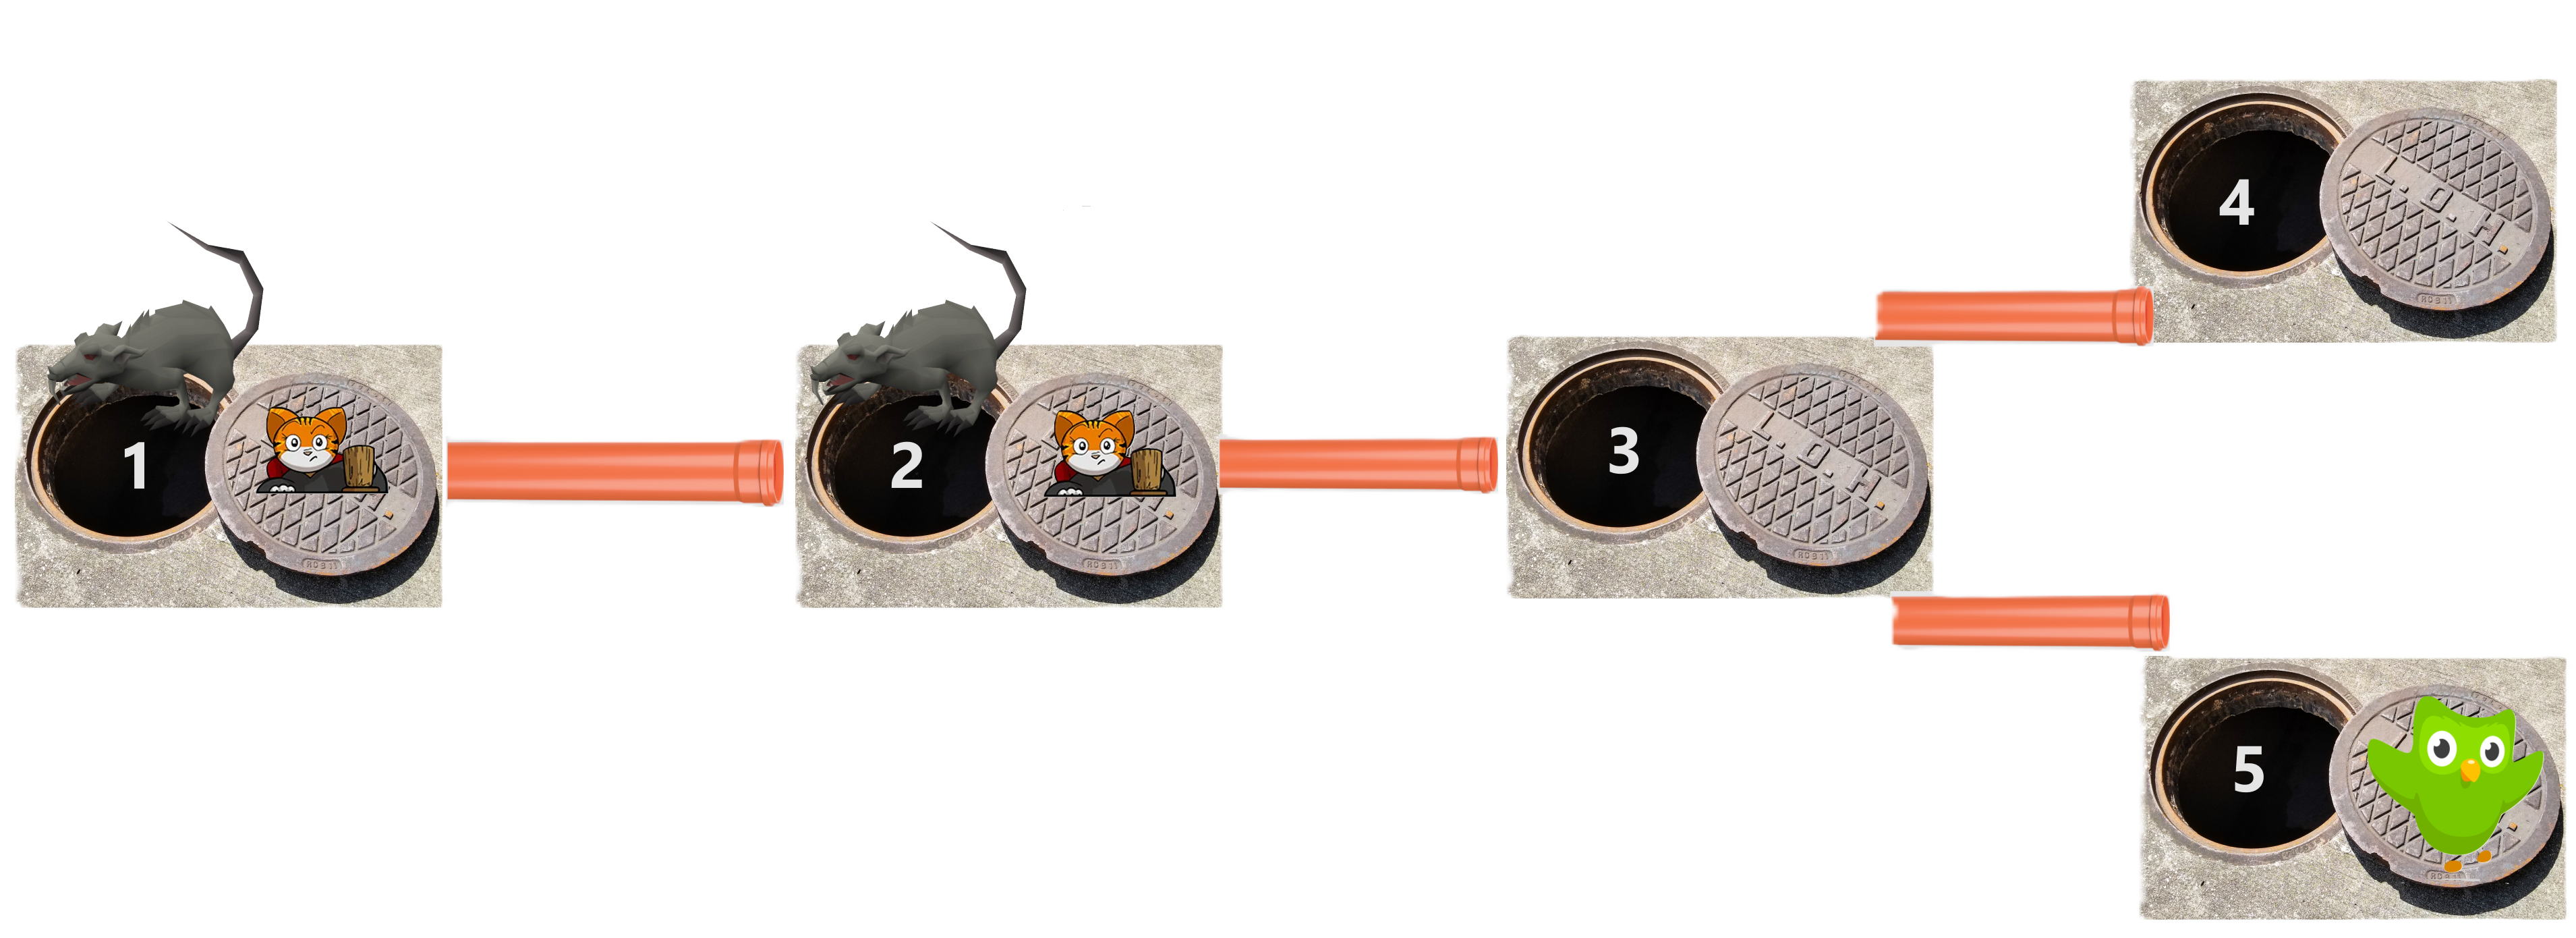
\includegraphics[scale=0.2]{rats_graph step3.png}
    \caption{När du ännu en gång placerar en ensam UGGL:a i brunn $5$ flyr först råttan i brunn $2$ till brunn $1$, och råttan i brunn $3$ flyr sedan till brunn $2$.}
  \end{figure}
\end{centering}

\begin{centering}
  \begin{figure}[h]
    \centering
    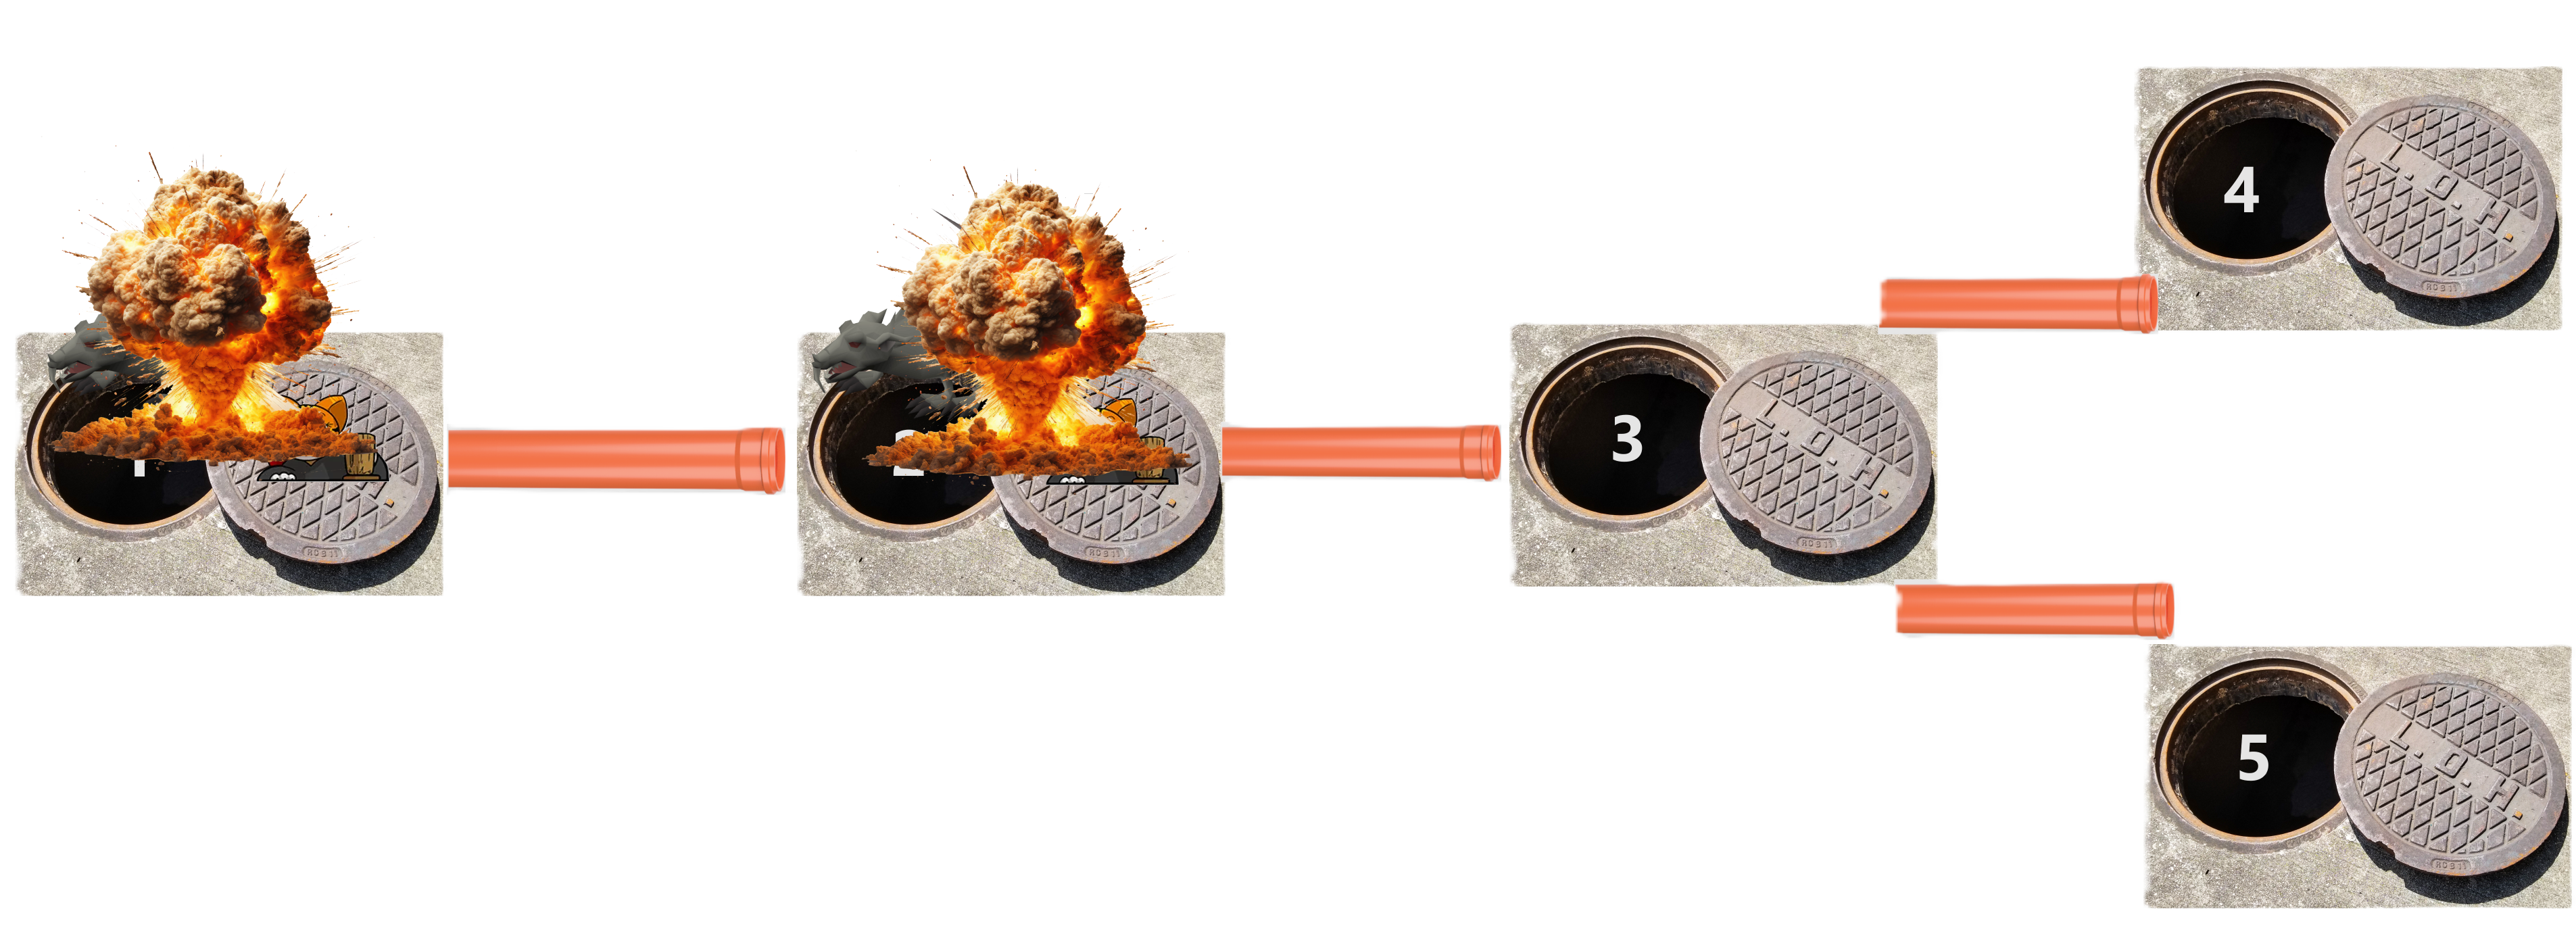
\includegraphics[scale=0.2]{rats_graph step4 activate.png}
    \caption{Nu är alla råttor i brunnar med KATT:er, och du kan aktivera KATT:erna.}
  \end{figure}
\end{centering}